

	\begin{multicols}{2}
		\section{Grundlage Projektierung}
			\textbf{Nutzungsvereinbarung} (SIA 260, S.19): Anforderungen an Nutzung definieren
				\begin{itemize}
					
					\item allgemeine Ziele für die Nutzung wie
					vorgesehene Nutzung, Nutzungsdauer etc.
					\item Umfeld und Drittanforderungen (z.B.
					Immissionen, Setzungen)
					\item Bedürfnisse des Betriebs und des Unterhalts
					\item Besondere Vorgaben der Bauherrschaft
					\item Schutzziele und Sonderrisiken
										
				\end{itemize}			
		
		\medskip
		
			\textbf{Projektbasis} (SIA 260, S.21): Bauwerksspezifische Umsetzung der
			Nutzungsvereinbarung
			\begin{itemize}
				
				\item Geplante Nutzungsdauer
				\item Nutzungszustände
				\item Gefährdungsbilder
				\item Anforderungen an Tragsicherheit, Gebrauchstauglichkeit und Dauerhaftigkeit sowie die vorgesehenen Massnahmen
				\item Akzeptierte Risiken
				
			\end{itemize}
		
	
	
			\subsection{Gefährdungsbilder, Nutzungszustände und Einwirkungen}
			
			• Gefährdungsbilder: kritischen
			Situationen für (Trag-)Sicherheit des
			Bauwerks
			
			• Nutzungszustände: kritischen
			Situationen für Gebrauchstauglichkeit
			(= Funktionstüchtigkeit, Komfort und
			Aussehen) des Bauwerks
			
			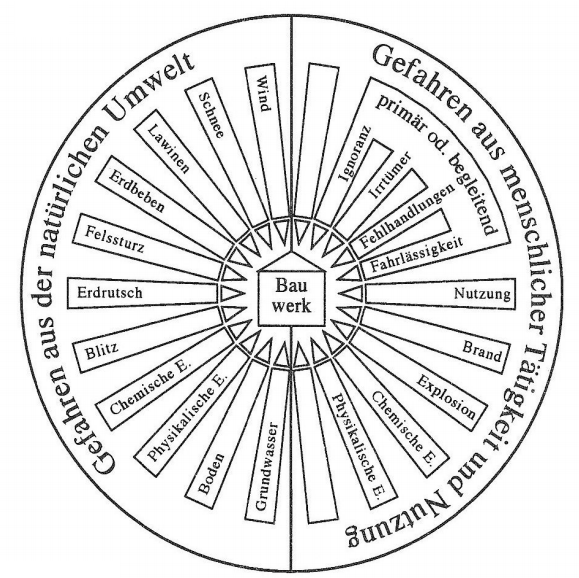
\includegraphics[width=\linewidth]{images/1Gefahren.PNG}
			
			
			\textbf{Gefährdungsanalyse:}
				\begin{enumerate}
					
					\item bestehende Erfahrungen  sammeln
					
					\item chronologisch Vorausdenken
					
					\item Nutzungsanalyse
					
					\item Einflussanalyse
					
					\item Energieanalyse
					
					\item Materialanalyse
					
					\item Brainstormin im interdisziplinären Team
					
					\item Logische Bäume (Fehler-, Ereignisbaum, Ursachen/Folgen)
					
					
				\end{enumerate}
			
			\medskip
			
			\textbf{Einwirkungen:} SIA 260 3.2 
			
			Einwirkungen: Norm SIA 261\\
			• Eigenlasten und Auflasten \\
			• Vorspannung \\
			• Baugrund \\
			• Schnee \\
			• Wind \\
			• Temperatur \\
			• Gebäudenutzung \\
			• Strassenverkehr \\
			• Normalspurbahnverkehr \\
			• Schmalspurbahnverkehr \\
			• Abschrankungen \\
			• Anprall \\
			• Brand \\
			• Erdbeben
			
			
			
			\subsection{Ständige Lasten}
			
			$\rightarrow$ Eigenlasten (Mittelwert, SIA 261 Anhang A) und Auflasten
			
			
			\subsection{Schnee}
			
			SIA 261, 5.1-4 $\rightarrow$ ortsfest, veränderlich
			
			
			\subsection{Wind}
			
			SIA 261, 6.1-3 $\rightarrow$ ortsfest, veränderlich
			
			
			\subsection{Temperatur}
			
			SIA 261, 7.1-2 $\rightarrow$ veränderlich
			
			\subsection{Gebäudenutzung}
			
			SIA 261, 8.1-4 $\rightarrow$ Nutzung durch Pers, Lastens des Mobiliars, Waren und Füllguts von Behältern, Leitungen, Einwirkungen von Maschinen und Fahrzeugen $\rightarrow$ frei veränderlich
			
			\subsection{Nichtmotorisierter Verkehr}
			
			SIA 261, 9.1-4
						
			\subsection{Strassenverkehr}
			
			SIA 261, 10.1-4 $\rightarrow$ frei veränderlich
			
			
			\subsection{Abschrankungen}
			
			SIA 261, 13.1-2 $\rightarrow$ veränderlich, gleichmässig verteilte horizontal Kräfte auf Höhe Handlauf
			
			
			\subsection{Anprall}
			
			SIA 261, 14.1-3 $\rightarrow$ aussergewöhnlich
			
			
				\subsection{Brand}
			
			SIA 261, 15.1-3 $\rightarrow$ Brandschutzziele in Nutzungsvereinbarung, Brandschutzkonzept in Projektbasis $\rightarrow$ aussergewöhnliche Leiteinwirkung
			
			
				\subsection{Erdbeben}
			
			SIA 261, 16.1-2 \& 16.5 \& 16.7 $\rightarrow$ aussergewöhnlich \\
			
			Entwurfsregeln:
				\begin{itemize}
					
					\item weiche Erdgeschosse vermeiden
					
					\item Unsymmetrische Aussteifungen (z.B. Wände) vermeiden (Verdrehung $\rightarrow$ Stützen knicken)
					
					\item zwei schlanke Stahlbetonwände pro Hauptrichtung (Länge: 1/5 bis 1/3 Gebäudehöhe, über ganze Höhe)
					
					\item Mischsysteme mit Stützen und tragenden Mauerwerkswänden vermeiden (Erdbebenkräfte von steifen Mauerwerkswänden aufgenommen $\rightarrow$ ungeeignet)
					
					\item Ausfachen von Rahmen durch Mauerwerk vermeiden
					
					\item Duktilen Bewehrungsstahl verwenden (grosser plastischer Bereich $\rightarrow$ Knautschzone)

					\item Keine Aussparungen und Öffnungen in
					plastischen Bereichen
					
					\item Tragwerk nicht auf stark unterschiedlich
					steifen Baugrund
					
					\item Einzelfundamente im Lockergestein		vermeiden oder untereinander durch Fundamentriegel usw. verbinden
					
					\item Fugen müssen eine ausreichende Breite besitzen, um das Zusammenstossen zweier benachbarter Blöcke zu vermeiden
					
					\item Höhenversatz vermeiden
					
				\end{itemize}
			
			
				\subsection{Bemessung}
			
			SIA 261, 4.1-3 \& 4.4 $\rightarrow$ Lastfälle def. (Leit-, veränderl. Begleiteinwirkung)
			
			
			
			
		
	\end{multicols}